\section{System Architecture}
This section will outline the technology stack we will use for the project. The system can be broken down into 3 layers. The presentation layer, the application layer and the data layer. Below we will highlight the different technologies used for each layer

\begin{figure}[h]
    \centering
    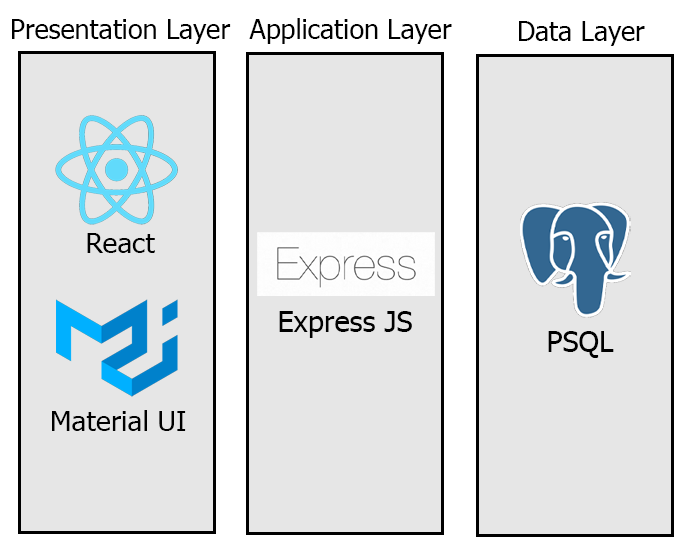
\includegraphics[scale=0.5]{architecture-layers}
    \caption{A visual breakdown of the different layers of our technology stack.}
\end{figure}

\subsection{Presentation Layer}
React will be used for the presentation layer, alongside the Material UI component library. React gas been chosen as its the current industry standard for front-end web design and can be easily used to develop high quality user experiences. Also many of our team members have had experience with using React in the past.\\
Material UI has been selected for a component library as its usage will make it very easy to standardise the visual style of our Meta LMS, as well as decreasing development time as it provides many high quality UI components that are ready to use. 

\subsection{Application Layer}
Express JS has been chosen to create our REST-API on the back-end due primarily to its ease of use, and the fact that having the front-end and the back-end written in the same language will make development easier for the entire team, as every member only has to be proficient in one programming language in order to work on all component of the project. Many of our team members already have experience with Express, and the PostgreSQL libraries for node also mean that using Express will simplify interactions between the API and the database.

\subsection{Data Layer}
A PostgreSQL has been selected for the Data layer due to its free and open source nature. It has also been selected based upon the experience of team members, as most of us have more experience with PostgreSQL over other database technologies.